\documentclass[11pt,letterpaper]{article}

% ============ DATOS DEL ESTUDIANTE ============
\newcommand{\nombreEstudiante}{Duván Felipe Baquero}
\newcommand{\codigoEstudiante}{160005002}
\newcommand{\nombreDocente}{Ángel Alfonso Cruz Roa}
% ==============================================

% Preámbulo agnóstico al motor: sirve con pdfLaTeX, XeLaTeX y LuaLaTeX.
\usepackage{iftex}
\ifPDFTeX
  \usepackage[utf8]{inputenc}
  \usepackage[T1]{fontenc}
  \usepackage{lmodern}
\else
  \usepackage{fontspec}
\fi

% babel-spanish redefine \% y rompe \,\% y el \% dentro de modo matemático.
\let\origpercent\%
\usepackage[spanish,es-tabla]{babel}
\AtBeginDocument{\let\%\origpercent}

\usepackage[margin=2.5cm]{geometry}
\usepackage{graphicx}
\usepackage{booktabs}
\usepackage{array}
\usepackage{makecell}
\usepackage{amsmath}
\usepackage{amssymb}
\usepackage{float}
\usepackage{xcolor}
\usepackage{fancyhdr}
\usepackage{caption}
\usepackage{enumitem}
\usepackage{microtype}
\usepackage{tocloft}
\usepackage[hidelinks]{hyperref}

\setlength{\cftbeforesecskip}{0.7em}
\captionsetup{font=small,labelfont=bf,skip=6pt}
\setlength{\parskip}{0.35em}
\renewcommand{\arraystretch}{1.12}

\pagestyle{fancy}
\fancyhf{}
\lhead{\small Universidad de los Llanos}
\rhead{\small Simulación Computacional --- Práctica N.\textsuperscript{o}\,02}
\rfoot{\small\thepage}
\renewcommand{\headrulewidth}{0.4pt}

\begin{document}

% =====================================================
% PORTADA
% =====================================================
\begin{titlepage}
\thispagestyle{empty}
\centering
\vspace*{\fill}

{\large \textsc{Universidad de los Llanos}}\\[0.2cm]
{\normalsize Facultad de Ciencias Básicas e Ingeniería}\\
{\normalsize Programa de Ingeniería de Sistemas}\\[1.6cm]

\rule{\textwidth}{0.8pt}\\[0.5cm]
{\LARGE \textbf{Números (pseudo)aleatorios y generación\\ de variables aleatorias}}\\[0.35cm]
{\large Generadores, pruebas de uniformidad y aleatoriedad,\\
integración Monte Carlo y simulación \emph{ad hoc} con\\
variables aleatorias Poisson y Binomiales}\\[0.5cm]
\rule{\textwidth}{0.8pt}\\[1.6cm]

{\normalsize Informe de la Práctica N.\textsuperscript{o}\,02}\\
{\normalsize Curso: Simulación Computacional}\\[1.4cm]

{\normalsize Presentado por:}\\[0.15cm]
{\large \nombreEstudiante}\\
{\normalsize Código: \codigoEstudiante}\\[1.2cm]

{\normalsize Docente:}\\[0.15cm]
{\large \nombreDocente}\\[1.6cm]

{\normalsize Villavicencio, Meta \\ \today}

\vspace*{\fill}
\end{titlepage}

\newpage
\tableofcontents
\newpage

% =====================================================
\section{Objetivos}
% =====================================================

Estos son los objetivos que trae la guía de laboratorio:

\begin{itemize}[itemsep=2pt]
    \item Introducir a los métodos para la generación y validación de números pseudoaleatorios.
    \item Generar secuencias de números pseudoaleatorios usando el método de MidSquare.
    \item Generar secuencias de números pseudoaleatorios usando el método del congruencial mixto.
    \item Generar secuencias de números pseudoaleatorios usando otros métodos.
    \item Calcular el tamaño de ciclo o periodo de una secuencia de números pseudoaleatorios.
    \item Evaluar si una secuencia de números pseudoaleatorios cumple con los criterios de uniformidad y aleatoriedad.
    \item Generar secuencias de valores de una variable aleatoria de una distribución de probabilidad discreta usando el método de la transformada inversa.
\end{itemize}

% =====================================================
\section{Consulta previa}
% =====================================================

\subsection{¿Qué es una variable aleatoria?}

Es una función que le asigna un número real a cada resultado posible de un experimento aleatorio.
Su utilidad está en que permite hacer cuentas con resultados que en sí mismos no son numéricos. Se
llama discreta cuando su conjunto de valores posibles es finito o numerable, y continua cuando puede
tomar cualquier valor de un intervalo de los reales. En esta práctica aparecen varias: el valor $X$
del numeral 5.3, y en el 5.4 el tiempo entre llegadas y el tiempo de servicio del cajero.

\subsection{¿Qué es una distribución de probabilidad?}

Es la regla que dice con qué probabilidad la variable aleatoria toma cada uno de sus valores
posibles. Para una variable discreta se describe con la función de masa $p_j = P\{X = j\}$, que
cumple $p_j \ge 0$ y $\sum_j p_j = 1$. Para una continua se describe con la función de densidad
$f(x)$, que cumple $f(x) \ge 0$ e integra 1 sobre todo su dominio. En ambos casos la función de
distribución acumulada es $F(x) = P\{X \le x\}$, y es la que se invierte en el método de la
transformada inversa.

\subsection{¿Cuál es la diferencia entre una distribución discreta y una continua?}

La discreta vive sobre un conjunto de valores separados y cada valor tiene una probabilidad positiva
propia, así que las probabilidades se suman. La continua puede tomar cualquier valor dentro de un
intervalo, la probabilidad de un punto exacto es cero y las probabilidades se calculan integrando la
densidad. La Poisson y la Binomial del numeral 5.4 son discretas. La $U(0,1)$ que intentan reproducir
los generadores del numeral 5.1 es continua, aunque en la práctica un computador solo puede producir
una versión discretizada de ella, con $m$ valores posibles como máximo.

\subsection{¿Cuál es la definición de la distribución uniforme continua $U(0,1)$?}

Es la distribución con densidad constante sobre el intervalo unitario:

\[
f(u) =
\begin{cases}
1, & 0 < u < 1,\\
0, & \text{en otro caso.}
\end{cases}
\]

Su acumulada es $F(u) = u$ dentro de $(0,1)$, su media vale $1/2$ y su varianza $1/12$. Es la
distribución de referencia de todo el laboratorio: los generadores del numeral 5.1 buscan producir
valores que se comporten como muestras suyas, y los numerales 5.2, 5.3 y 5.4 los usan como materia
prima.

\subsection{¿Cuál es la definición de la distribución de Poisson?}

Una variable aleatoria $X$ sigue una distribución de Poisson de media $\lambda$ si

\[
p_i = P\{X = i\} = e^{-\lambda}\,\frac{\lambda^i}{i!}, \qquad i = 0, 1, 2, \dots
\]

Tiene la particularidad de que su media y su varianza valen las dos $\lambda$. Cumple además la
recursión $p_{i+1} = \frac{\lambda}{i+1}p_i$, que es la que aprovecha el algoritmo de generación de
la sección 4.2 de \cite{ross99} para no calcular factoriales.

\subsection{¿Cuál es la definición de la distribución Binomial?}

Una variable $X$ es Binomial de parámetros $n$ y $p$ si cuenta el número de éxitos en $n$ ensayos
independientes, cada uno con probabilidad $p$ de éxito:

\[
P\{X = i\} = \binom{n}{i} p^i (1-p)^{n-i}, \qquad i = 0, 1, \dots, n.
\]

Su media es $np$ y su varianza $np(1-p)$. También tiene recursión propia,
$P\{X = i+1\} = \frac{n-i}{i+1}\cdot\frac{p}{1-p}\,P\{X = i\}$, y con $n = 10$ y $p = 0{,}40$ da
media 4 y varianza 2,4.

\subsection{¿A qué se refiere que una variable aleatoria sea i.i.d.?}

A que las observaciones de una sucesión salgan todas de la misma distribución y que ninguna dependa
de las anteriores. Es exactamente lo que se le exige a un generador de números pseudoaleatorios, y
por eso hay que aplicarle dos tipos de prueba distintos: la de uniformidad revisa la parte de
idénticamente distribuidas y la de rachas revisa la de independientes. El generador de congruencia
inversa del numeral 5.1 resultó ser un buen ejemplo de que se puede cumplir lo primero de manera casi
perfecta y fallar lo segundo.

\subsection{¿En qué consiste una prueba o test estadístico?}

Es un procedimiento para decidir si lo que se observó es compatible con una hipótesis. Se plantea una
hipótesis nula $H_0$, se calcula un estadístico a partir de la muestra y se compara contra un valor
crítico que depende del nivel de significancia $\alpha$, que es la probabilidad de rechazar $H_0$
siendo cierta. Si el estadístico supera el valor crítico se rechaza. En este laboratorio se usan tres
pruebas, todas con $\alpha = 0{,}05$: Kolmogorov--Smirnov y $\chi^2$ para uniformidad, y el test de
rachas para aleatoriedad.

% =====================================================
\section{Metodología y herramientas}
% =====================================================

Todo el desarrollo está en un único cuaderno de Jupyter en Python, ejecutado de principio a fin y
adjunto a este informe:

\begin{center}
\texttt{Lab2\_Simulacion\_Duvan\_Baquero\_\codigoEstudiante.ipynb}
\end{center}

Se usan solamente \texttt{numpy}, \texttt{pandas}, \texttt{matplotlib} y \texttt{scipy}, que ya
vienen instalados en Google Colab.

Los generadores no se tomaron de ninguna librería. El congruencial mixto, el MidSquare, el
\emph{shift-register}, el de congruencia inversa, la transformada inversa discreta, el método de
composición y los generadores de Poisson y Binomial están escritos a mano siguiendo los algoritmos de
los capítulos 3 y 4 de \cite{ross99}. De \texttt{scipy} solo se usan los valores críticos de las
distribuciones $\chi^2$ y normal, las funciones de masa teóricas contra las que se comparan las
frecuencias observadas y una cuadratura numérica para tener un valor de referencia en tres de las
siete integrales del numeral 5.2.

Como todos los generadores son deterministas y las semillas están fijas en el código, cualquier
persona que ejecute el cuaderno obtiene exactamente las mismas tablas que aparecen aquí.

% =====================================================
\section{Numeral 5.1: generación de números (pseudo)aleatorios}
% =====================================================

\subsection{Los tres métodos implementados}

\textbf{MidSquare.} Eleva el estado al cuadrado, lo rellena con ceros a la izquierda hasta $2D$
dígitos y toma los $D$ centrales como estado siguiente, con $u_i = X_i/10^{D}$. Se corrió con las
cinco semillas de la guía: 1931, 675248, 4567, 12122 y 7179345.

\textbf{Congruencial mixto.} Aplica $X_{n+1} = (a X_n + c) \bmod m$ y normaliza con $u_i = X_i/m$. Se
corrieron los cinco juegos de parámetros de la guía, que van desde un módulo de 48 hasta $2^{48}$.

\textbf{Otros dos generadores.} De la lista del artículo de \cite{mancilla2000} escogí el
\emph{shift-register} y el de congruencia inversa. El primero es un registro de desplazamiento de
$k = 7$ bits con realimentación $b_i = b_{i-k} \oplus b_{i-1}$, del que se toman bloques de $w = 8$
bits para formar cada número. El segundo usa $X_{n+1} = (a X_n^{-1} + b) \bmod m$ con $m = 101$,
$a = 2$ y $b = 7$, donde $X^{-1}$ es el inverso multiplicativo módulo $m$.

Cada método produjo secuencias de $n = 100$ números, doce secuencias en total.

\subsection{Periodo y pruebas de uniformidad y aleatoriedad}

El periodo se obtuvo recorriendo la sucesión de estados y guardando la primera aparición de cada uno.
Al encontrar un estado repetido quedan determinadas la cola $\mu$, que es el transitorio antes de
entrar al ciclo, y el periodo $\lambda$. Para los dos módulos grandes del congruencial mixto la
búsqueda no es viable y se reporta el periodo teórico.

La uniformidad se probó con Kolmogorov--Smirnov como prueba principal y $\chi^2$ con 10 clases como
verificación. La aleatoriedad, con el test de rachas ascendentes y descendentes. Los valores críticos
para $n = 100$ y $\alpha = 0{,}05$ son $D_{0,05} = 0{,}1340$, $\chi^2_{9;\,0,95} = 16{,}919$ y
$|Z| = 1{,}96$. La tabla \ref{tab:res51} reúne los resultados.

\begin{table}[H]
\centering
\caption{Periodo y resultado de las tres pruebas para las doce secuencias generadas.}
\label{tab:res51}
\footnotesize\setlength{\tabcolsep}{4pt}
\begin{tabular}{@{}llrrrcrcrc@{}}
\toprule
Punto & Generador & $\lambda$ & $\mu$ & $D$ & KS & $\chi^2$ & $\chi^2$ & $Z$ & Rachas \\
\midrule
5.1.1 & MidSquare $X_0=1931$    & 1 & 7   & 0,9740 & FALLA & 860,6 & FALLA & $-15{,}64$ & FALLA \\
5.1.1 & MidSquare $X_0=675248$  & 1 & 210 & 0,0820 & PASA  & 12,4  & PASA  & 0,88       & PASA  \\
5.1.1 & MidSquare $X_0=4567$    & 4 & 19  & 0,1700 & FALLA & 109,4 & FALLA & $-4{,}39$  & FALLA \\
5.1.1 & MidSquare $X_0=12122$   & 1 & 88  & 0,2166 & FALLA & 52,2  & FALLA & $-3{,}19$  & FALLA \\
5.1.1 & MidSquare $X_0=7179345$ & 20 & 848 & 0,1043 & PASA & 15,0  & PASA  & $-0{,}08$  & PASA  \\
\addlinespace
5.1.2 & GLC a) $m=128$          & 32 & 0 & 0,0441 & PASA  & 6,8  & PASA  & 0,64      & PASA \\
5.1.2 & GLC b) $m=48$           & 48 & 0 & 0,0358 & PASA  & 1,2  & PASA  & 1,12      & PASA \\
5.1.2 & GLC c) $m=2^{31}-1$     & \multicolumn{1}{c}{$2{,}1\times10^{9}$} & 0 & 0,1452 & FALLA & 12,0 & PASA & $-0{,}56$ & PASA \\
5.1.2 & GLC d) $m=2^{48}$       & \multicolumn{1}{c}{$2{,}8\times10^{14}$} & 0 & 0,0831 & PASA & 4,8 & PASA & $-0{,}80$ & PASA \\
5.1.2 & GLC e) $m=200$          & 8 & 2 & 0,0950 & PASA  & 22,8 & FALLA & 1,84      & PASA \\
\addlinespace
5.1.3 & Shift-Register $k=7$    & 127 & 0 & 0,0369 & PASA & 1,0 & PASA & 0,16 & PASA  \\
5.1.3 & Congruencia inversa     & 101 & 0 & 0,0099 & PASA & 0,0 & PASA & 2,31 & FALLA \\
\bottomrule
\end{tabular}
\begin{minipage}{\textwidth}\vspace{2pt}\footnotesize
Valores críticos con $n=100$ y $\alpha=0{,}05$: $D_{0,05}=0{,}1340$, $\chi^2_{9;\,0,95}=16{,}919$ y
$|Z|=1{,}96$. Los periodos de los literales c) y d) son los teóricos, ya que su búsqueda directa no
es viable.
\end{minipage}
\end{table}

Antes de responder las preguntas hay que señalar algo que se ve en esa tabla y que cambia la lectura
por completo. Un generador con periodo $\lambda \le n = 100$ recorre su ciclo entero dentro de la
muestra, y al enumerar todos sus estados un número exacto de veces produce un histograma
perfectamente plano. Los literales a) y b) del congruencial mixto pasan las tres pruebas por esa
razón, no porque sean buenos. El tamaño de ciclo hay que mirarlo antes que las pruebas, no después.

\subsection{¿Cuáles son los peores generadores y por qué?}

El peor de todos es el MidSquare con $X_0 = 1931$. A las siete iteraciones cae en el estado cero y de
ahí no sale: su periodo es $\lambda = 1$ y 93 de los 100 valores generados son exactamente 0. Falla
las tres pruebas de forma escandalosa, con $D = 0{,}9740$ contra un crítico de 0,1340 y
$\chi^2 = 860{,}6$ contra 16,919. No es un generador de números aleatorios, es una constante.

Los otros dos MidSquare que fallan sufren la misma enfermedad en distinto grado. El de
$X_0 = 12122$ degenera a cero en la iteración 88, y el de $X_0 = 4567$ entra en el ciclo corto
$4100 \to 8100 \to 6100 \to 2100$ de periodo 4, de modo que 82 de sus 100 valores son apenas cuatro
números repitiéndose.

El congruencial mixto e), con $X_0 = 3$, $a = 5$, $c = 7$ y $m = 200$, tiene periodo 8. En 100
números produce solo 9 valores distintos. No cumple las condiciones de Hull--Dobell porque
$m = 200 = 2^3 \cdot 5^2$ es divisible por 5 pero $a - 1 = 4$ no lo es. Lo curioso es que pasa el
Kolmogorov--Smirnov con $D = 0{,}0950$, y aun así el $\chi^2$ lo rechaza con 22,8 porque quedan
clases con frecuencia 0 y 1 mientras otras tienen 12 o 13. Es la mejor prueba de que pasar un
contraste de uniformidad con periodo 8 no significa nada.

Los literales a) y b) del congruencial mixto son malos por periodo aunque pasen las tres pruebas. Sus
ciclos son de 32 y 48, menores que la muestra. El caso a) además usa $c = 0$ con $m = 2^7$, y un
generador multiplicativo con módulo potencia de dos tiene periodo máximo $m/4 = 32$, que es
justamente el que se obtuvo.

Caso aparte es el de congruencia inversa. Tiene periodo completo $\lambda = m = 101$ y la mejor
uniformidad del laboratorio, con $D = 0{,}0099$ y $\chi^2 = 0{,}0$, es decir exactamente 10
observaciones en cada una de las 10 clases. Pero falla el test de rachas con $R = 76$ frente a las
66,33 esperadas y $Z = 2{,}31$. Ese exceso de rachas indica alternancia entre valores altos y bajos:
los números están perfectamente repartidos pero no llegan en orden aleatorio. Es el ejemplo más claro
del laboratorio de que uniformidad y aleatoriedad son propiedades distintas.

\subsection{¿Cuáles son los mejores generadores y por qué?}

El mejor es el congruencial mixto d), con $X_0 = 29022024$, $a = 25214903917$, $c = 11$ y
$m = 2^{48}$. Es el único que junta las tres virtudes. Su periodo es el máximo posible,
$\lambda = m = 2^{48} \approx 2{,}8 \times 10^{14}$, porque cumple las tres condiciones de
Hull--Dobell: $\gcd(11, 2^{48}) = 1$, el único factor primo de $m$ es 2 y divide a $a-1 = 25214903916$,
y como $4 \mid m$ también $4 \mid (a-1)$. Pasa los dos contrastes de uniformidad con holgura
($D = 0{,}0831$ contra 0,1340; $\chi^2 = 4{,}8$ contra 16,919) y el de rachas con $Z = -0{,}80$. Es
el generador que usan \texttt{java.util.Random} y \texttt{drand48()} de C, y por eso es el que escogí
como fuente de números aleatorios para el numeral 5.2.

El \emph{shift-register} queda segundo. Alcanza el periodo máximo de su registro,
$\lambda = 2^7 - 1 = 127$ bits, y pasa las tres pruebas con muy buenos márgenes: $D = 0{,}0369$,
$\chi^2 = 1{,}0$ y $R = 67$ con $Z = 0{,}16$, que es prácticamente el número de rachas esperado. Su
limitación es de escala y no de calidad, porque con $k = 7$ el periodo es corto, pero eso se arregla
subiendo $k$ sin tocar el algoritmo.

El congruencial mixto c), que es el MINSTD de Lehmer, tiene periodo $\lambda = m - 1 = 2\,147\,483\,646$,
el máximo alcanzable por un generador multiplicativo, porque $m = 2^{31}-1$ es primo de Mersenne y
$a = 16807 = 7^5$ es raíz primitiva módulo $m$. Pasa el $\chi^2$ y el test de rachas, y falla el
Kolmogorov--Smirnov por muy poco, con $D = 0{,}1452$ contra el crítico 0,1340. Con
$\alpha = 0{,}01$ el crítico sube a 0,1607 y se aceptaría, así que el rechazo se explica por la
variabilidad de una muestra de apenas 100 números y no por un defecto de fondo.

Los dos MidSquare que pasaron las pruebas lo hicieron por suerte. Siguiendo la secuencia más allá de
los 100 valores se ve que el de $X_0 = 7179345$ cae en un ciclo de periodo 20 después de 848
iteraciones, y el de $X_0 = 675248$ degenera a cero en la iteración 210. Los buenos resultados se
deben únicamente a que la muestra se cortó antes de que apareciera el problema.

% =====================================================
\section{Numeral 5.2: uso de números aleatorios para evaluar integrales}
% =====================================================

\subsection{Planteamiento}

Si $U \sim U(0,1)$ entonces $\theta = \int_0^1 g(x)\,dx = E[g(U)]$, así que basta con generar
$u_1, \dots, u_k$ y promediar $g(u_i)$. Cuando los límites no son 0 y 1 hay que llevar la integral a
ese intervalo. La sección 3.2 de \cite{ross99} da los dos cambios de variable necesarios:

\[
\int_a^b g(x)\,dx = \int_0^1 (b-a)\,g\big(a + (b-a)y\big)\,dy,
\qquad
\int_0^{\infty} g(x)\,dx = \int_0^1 \frac{g\!\left(\frac{1}{y}-1\right)}{y^2}\,dy .
\]

Aplicados a los siete ejercicios, el ejercicio 5 se resuelve con $x = -2 + 4y$, los ejercicios 6 y 7
con $x = 1/y - 1$, y en el 7 se usa primero la simetría del integrando para escribir
$\int_{-\infty}^{\infty} e^{-x^2}dx = 2\int_0^{\infty} e^{-x^2}dx$.

El ejercicio 9 es el único que necesita la sugerencia de la guía. Definiendo $I_y(x) = 1$ si $y < x$ y
0 en caso contrario, el límite superior variable desaparece:

\[
\int_0^{\infty}\!\!\int_0^{x} e^{-(x+y)}\,dy\,dx
= \int_0^{\infty}\!\!\int_0^{\infty} e^{-(x+y)}\,I_y(x)\,dy\,dx ,
\]

y ahora las dos variables van de 0 a infinito, así que se les aplica la misma sustitución a las dos.

Como fuente de los $u_i$ usé el congruencial mixto d) del numeral 5.1.2, el mejor calificado en el
5.1.4. Solo para llenar la tabla siguiente se consumieron 999\,900 números, mucho más que el periodo
de siete de los doce generadores evaluados, lo cual justifica la elección.

\subsection{Resultados}

\begin{table}[H]
\centering
\caption{Estimaciones Monte Carlo de los ejercicios 3 a 9 con distintos tama\~nos de muestra.}
\label{tab:int}
\small\setlength{\tabcolsep}{4pt}
\begin{tabular}{@{}clrrrrrr@{}}
\toprule
Ej. & Integral & Exacto & $k=100$ & $k=10^3$ & $k=10^4$ & $k=10^5$ & \makecell{Error rel.\\$k=10^5$} \\
\midrule
3 & $\int_0^1 \exp\{e^x\}\,dx$ & 6,3166 & 6,4649 & 6,2780 & 6,3114 & 6,3140 & 0,041\% \\
4 & $\int_0^1 (1-x^2)^{3/2}\,dx$ & 0,5890 & 0,5967 & 0,5866 & 0,5890 & 0,5901 & 0,186\% \\
5 & $\int_{-2}^{2} e^{x+x^2}\,dx$ & 93,1628 & 29,2253 & 87,7549 & 94,8579 & 93,6161 & 0,487\% \\
6 & $\int_0^{\infty} x(1+x^2)^{-2}\,dx$ & 0,5000 & 0,5338 & 0,5185 & 0,4962 & 0,5012 & 0,232\% \\
7 & $\int_{-\infty}^{\infty} e^{-x^2}\,dx$ & 1,7725 & 1,9186 & 1,8210 & 1,7800 & 1,7758 & 0,187\% \\
8 & $\int_0^1\!\!\int_0^1 e^{(x+y)^2}\,dy\,dx$ & 4,8992 & 5,6867 & 4,7126 & 4,8674 & 4,9053 & 0,125\% \\
9 & $\int_0^{\infty}\!\!\int_0^{x} e^{-(x+y)}\,dy\,dx$ & 0,5000 & 0,5625 & 0,4839 & 0,5002 & 0,4991 & 0,174\% \\
\bottomrule
\end{tabular}
\end{table}

\begin{table}[H]
\centering
\caption{Error relativo porcentual de cada estimaci\'on seg\'un el tama\~no de muestra.}
\label{tab:interr}
\small
\begin{tabular}{@{}crrrr@{}}
\toprule
Ejercicio & $k=100$ & $k=1\,000$ & $k=10\,000$ & $k=100\,000$ \\
\midrule
3 & 2,35\% & 0,61\% & 0,083\% & 0,041\% \\
4 & 1,31\% & 0,42\% & 0,015\% & 0,186\% \\
5 & 68,63\% & 5,80\% & 1,820\% & 0,487\% \\
6 & 6,77\% & 3,69\% & 0,751\% & 0,232\% \\
7 & 8,24\% & 2,74\% & 0,425\% & 0,187\% \\
8 & 16,08\% & 3,81\% & 0,647\% & 0,125\% \\
9 & 12,51\% & 3,21\% & 0,036\% & 0,174\% \\
\bottomrule
\end{tabular}
\end{table}

\begin{figure}[H]
\centering
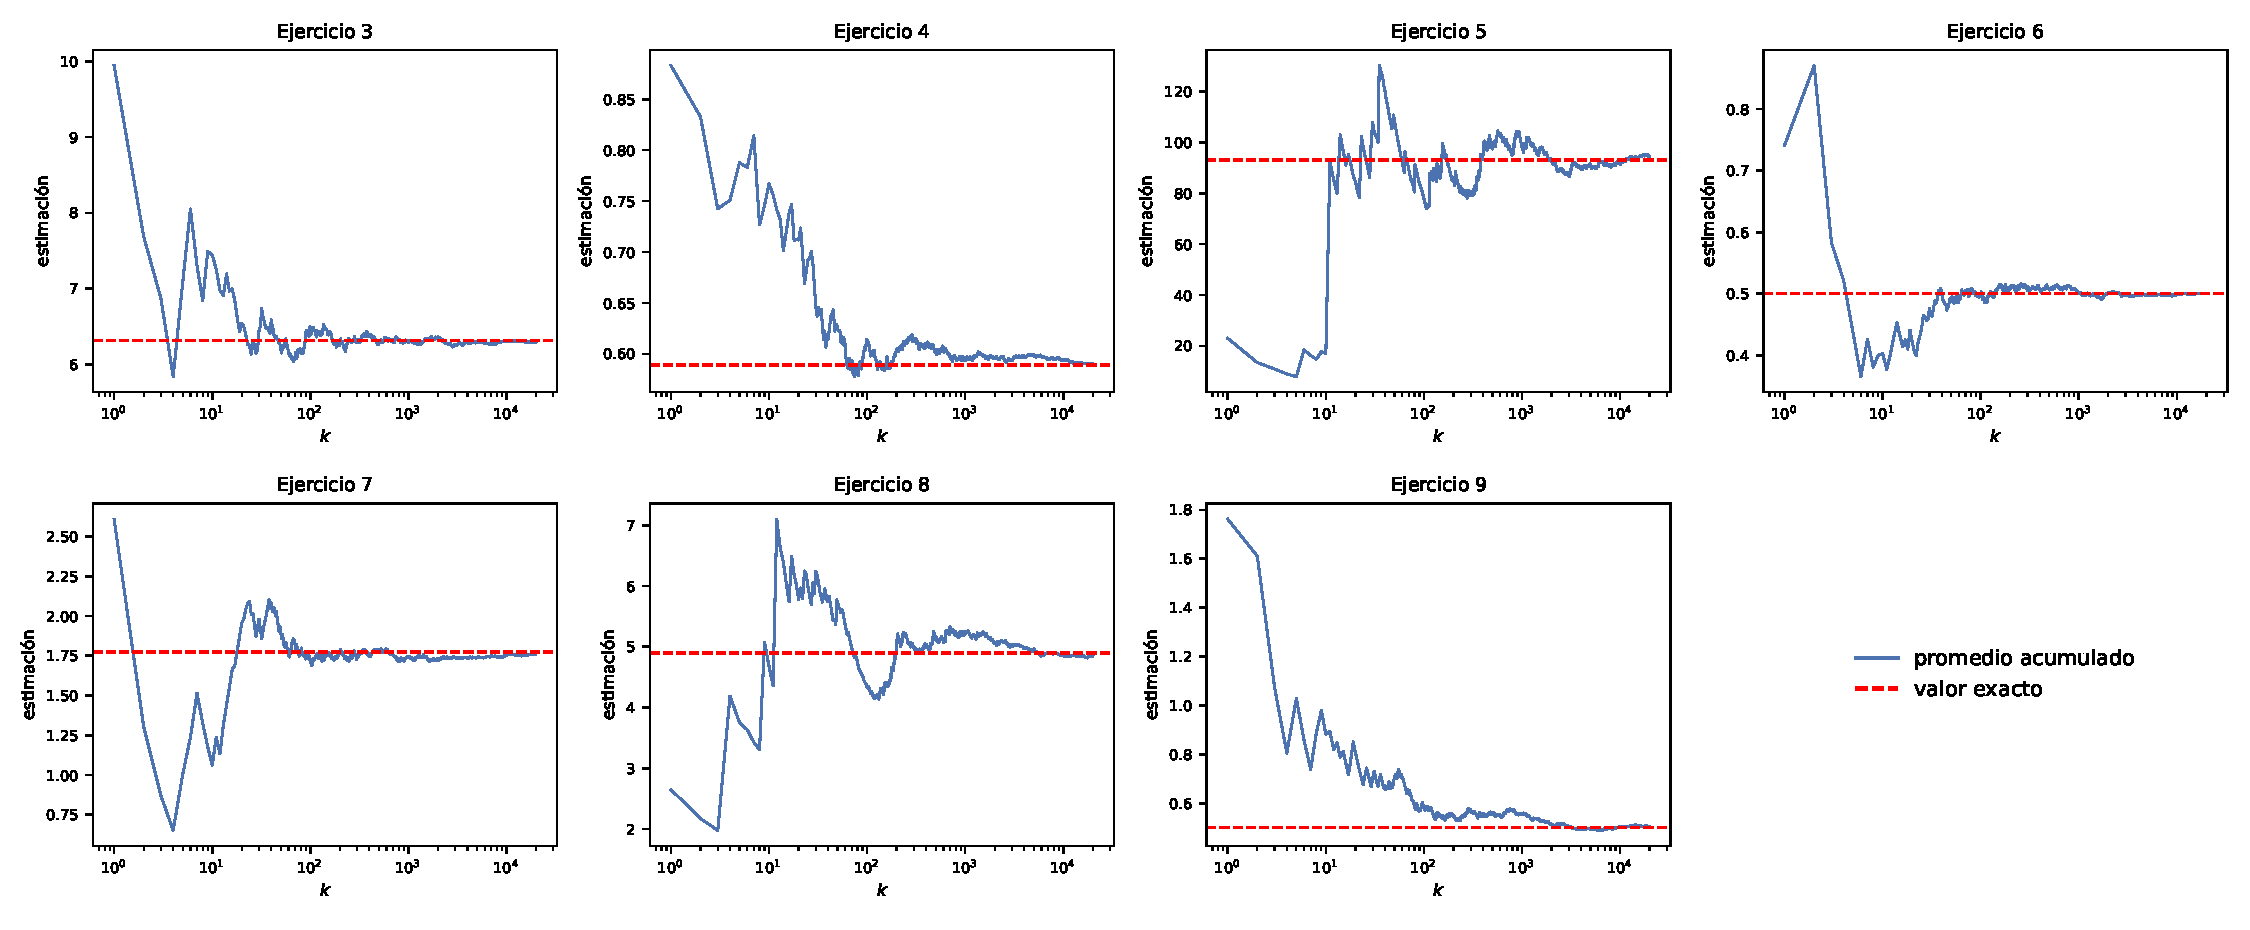
\includegraphics[width=\textwidth]{fig_convergencia.pdf}
\caption{Promedio acumulado de cada estimador frente al valor exacto, con el eje horizontal en escala
logarítmica.}
\label{fig:conv}
\end{figure}

\subsection{Análisis}

Con $k = 100\,000$ los siete estimadores quedan por debajo del 0,5\,\% de error relativo, y el
promedio de los siete es 0,20\,\%. Lo interesante está en las muestras pequeñas.

El ejercicio 5 es el caso extremo. Con 100 números la estimación fue 29,23 frente al valor real
93,16, un error del 68,6\,\%. La razón está en el integrando: sobre $[-2,2]$, la función $e^{x+x^2}$
vale 0,78 en su mínimo y 403,4 en $x = 2$. Un puñado de puntos cerca del extremo derecho decide casi
todo el promedio, y si en 100 sorteos ninguno cae ahí la estimación se queda corta. Con $k = 1\,000$
el error baja a 5,80\,\% y con $k = 100\,000$ a 0,49\,\%.

Los ejercicios 8 y 9 arrancan con errores de 16,08\,\% y 12,51\,\%. En el 9 el motivo es distinto al
del 5: el indicador $I_y(x)$ anula aproximadamente la mitad de las evaluaciones, así que de 100 pares
solo unos 50 aportan información. El ejercicio 4 es el que mejor se porta desde el comienzo, con
1,31\,\% de error usando apenas 100 números, porque su integrando es suave y está acotado entre 0 y 1.

El patrón general de la figura \ref{fig:conv} es que el error cae como $1/\sqrt{k}$. Multiplicar la
muestra por 100 reduce el error unas 10 veces y no 100. Entre $k=100$ y $k=10\,000$ el error del
ejercicio 3 pasó de 2,35\,\% a 0,083\,\%, y el del ejercicio 7 de 8,24\,\% a 0,43\,\%. Esa lentitud
es el precio del método Monte Carlo.

Una observación de implementación: los ejercicios 6, 7 y 9 dividen entre $u^2$, de modo que un $u_i$
muy cercano a cero produce un valor enorme. Con $m = 2^{48}$ el generador nunca devuelve cero exacto y
el problema no llegó a presentarse, pero es la razón de que esos tres estimadores tengan más varianza
que los demás.

% =====================================================
\section{Numeral 5.3: generación de variables aleatorias discretas}
% =====================================================

El método de la transformada inversa discreta parte el intervalo unitario en pedazos cuyas longitudes
son las probabilidades $p_j$, y devuelve el valor cuyo pedazo contiene al número aleatorio:
$X = j$ si $F(j-1) \le U < F(j)$. Todo este numeral usa el generador congruencial mixto que exige la
guía, con $X_0 = 2391$, $a = 25214903917$, $c = 11$ y $m = 2^{48}$. Cada literal vuelve a arrancar en
$X_0 = 2391$, así que los cuatro parten de la misma sucesión $u_1, \dots, u_{100}$ y lo único que
cambia entre uno y otro es cómo se parte $(0,1)$.

\subsection{Literales a) y b)}

En el literal a) las probabilidades son 0,20, 0,15, 0,25 y 0,40, con cortes en 0,20, 0,35 y 0,60.
Este caso es literalmente el Ejemplo 4a del capítulo 4 de \cite{ross99}. En el literal b) son 0,30,
0,20, 0,35 y 0,15, con cortes en 0,30, 0,50 y 0,85. Los 100 valores de cada uno aparecen en el
cuaderno; aquí van las frecuencias.

\begin{table}[H]
\centering
\caption{Frecuencias observadas en los 100 valores generados en los literales a) y b).}
\label{tab:53ab}
\small
\begin{tabular}{@{}crrr@{\hspace{2em}}rrr@{}}
\toprule
& \multicolumn{3}{c}{Literal a)} & \multicolumn{3}{c}{Literal b)} \\
\cmidrule(lr){2-4}\cmidrule(lr){5-7}
$X=j$ & $p_j$ & Obs. & Esp. & $p_j$ & Obs. & Esp. \\
\midrule
1 & 0,20 & 21 & 20 & 0,30 & 32 & 30 \\
2 & 0,15 & 14 & 15 & 0,20 & 22 & 20 \\
3 & 0,25 & 27 & 25 & 0,35 & 29 & 35 \\
4 & 0,40 & 38 & 40 & 0,15 & 17 & 15 \\
\midrule
Total & 1,00 & 100 & 100 & 1,00 & 100 & 100 \\
\bottomrule
\end{tabular}
\begin{minipage}{\textwidth}\vspace{2pt}\footnotesize
Literal a): $\chi^2 = 0{,}3767$. Literal b): $\chi^2 = 1{,}6286$. Valor cr\'itico con 3 grados de libertad y $\alpha=0{,}05$: $7{,}8147$.
\end{minipage}
\end{table}

Los dos ajustan bien. Con tres grados de libertad y $\alpha = 0{,}05$ el valor crítico es 7,8147, y
los estadísticos obtenidos fueron 0,3767 y 1,6286.

Hay un detalle que me pareció revelador. Los dos literales usan exactamente los mismos 100 números
$u_i$ y aun así 51 de los 100 valores generados son distintos. Solo cambió la partición del
intervalo. Eso deja claro que el generador y la variable aleatoria son dos piezas separadas: uno
produce la materia prima uniforme y el otro la moldea.

El libro también propone, para el mismo literal a), una versión más eficiente que revisa las clases
de mayor a menor probabilidad: primero si $u < 0{,}40$ para $X = 4$, luego $u < 0{,}65$ para $X = 3$,
luego $u < 0{,}85$ para $X = 1$ y si no $X = 2$. Implementé las dos para poder medir la diferencia. En
el literal a) el orden natural cuesta 2,82 comparaciones por valor generado y el orden decreciente
2,11, un ahorro del 25,2\,\%. En el literal b) el ahorro es de apenas 6,1\,\%, de 2,31 a 2,17, porque
ahí las cuatro probabilidades están más parejas y la mayor, 0,35, no domina tanto. Aclaro
que las dos versiones no producen los mismos 100 valores aunque sí la misma distribución, porque al
reordenar los subintervalos a cada $u_i$ le toca otro valor de $X$.

\subsection{Literal c)}

Con solo dos valores la transformada inversa se reduce a una comparación: $X = 1$ si $u < 1/3$ y
$X = 2$ en caso contrario.

\begin{table}[H]
\centering
\caption{Literal c): proporci\'on de valores iguales a 1 con $p_1 = 1/3$.}
\label{tab:53c}
\small
\begin{tabular}{@{}rrrrrr@{}}
\toprule
$n$ & Unos & Proporci\'on & Te\'orico & Diferencia & Diferencia/EE \\
\midrule
100 & 34 & 0,3400 & 0,3333 & +0,0067 & +0,141 \\
1000 & 328 & 0,3280 & 0,3333 & -0,0053 & -0,358 \\
10000 & 3316 & 0,3316 & 0,3333 & -0,0017 & -0,368 \\
\bottomrule
\end{tabular}
\end{table}

La proporción se acerca al valor teórico $1/3$ conforme crece $n$, y la diferencia absoluta baja de
0,0067 a 0,0017. Midiéndola en errores estándar, las tres desviaciones quedan por debajo de 0,4, así
que ninguna es sospechosa. El error estándar teórico $\sqrt{p(1-p)/n}$ pasa de 0,0471 a 0,0047, otra
vez la caída como $1/\sqrt{n}$ que ya se había visto en el numeral 5.2. Como las tres corridas
arrancan en la misma semilla, la de $n = 1\,000$ contiene a la de $n = 100$ en sus primeras 100
observaciones.

\subsection{Literal d): método de composición}

Las probabilidades son 0,06 para $j = 1,\dots,5$ y 0,15, 0,13, 0,14, 0,15, 0,13 para $j = 6,\dots,10$.
Todas valen al menos 0,06, y esa es la pista para descomponerlas como en el Ejemplo 4f del libro:

\[
p_j = \alpha\,p_j^{1} + (1-\alpha)\,p_j^{2}, \qquad \alpha = 0{,}6,
\]

con $p_j^{1} = 0{,}1$ para todo $j$, que es la uniforme discreta en $1,\dots,10$. Despejando queda
$p_j^{2} = (p_j - 0{,}06)/0{,}4$, es decir

\[
p^{2} = (0,\ 0,\ 0,\ 0,\ 0,\ 0{,}225,\ 0{,}175,\ 0{,}200,\ 0{,}225,\ 0{,}175).
\]

Los cinco primeros se anulan porque $0{,}6 \times 0{,}1 = 0{,}06$ es toda su probabilidad. Escogí
$\alpha = 0{,}6$ por ser el valor más grande que deja las diez componentes de $p^{2}$ no negativas, y
mientras más grande sea $\alpha$ más seguido se resuelve el sorteo por la rama barata.

El algoritmo queda así:

\begin{quote}
\textsc{Paso 1:} generar un número aleatorio $U_1$.\\
\textsc{Paso 2:} generar un número aleatorio $U_2$.\\
\textsc{Paso 3:} si $U_1 < 0{,}6$, hacer $X = \mathrm{Ent}(10\,U_2) + 1$ y terminar. En caso
contrario, aplicar la transformada inversa sobre $p^{2}$, que solo tiene masa en $6,\dots,10$,
revisando de mayor a menor probabilidad.
\end{quote}

\begin{table}[H]
\centering
\caption{Literal d): descomposici\'on y ajuste de 10\,000 valores generados por composici\'on.}
\label{tab:53d}
\small
\begin{tabular}{@{}crrrrrr@{}}
\toprule
$X=j$ & $p_j$ & $p_j^{1}$ & $p_j^{2}$ & Observada & Esperada & Frec. rel. \\
\midrule
1 & 0,06 & 0,10 & 0,000 & 577 & 600 & 0,0577 \\
2 & 0,06 & 0,10 & 0,000 & 627 & 600 & 0,0627 \\
3 & 0,06 & 0,10 & 0,000 & 586 & 600 & 0,0586 \\
4 & 0,06 & 0,10 & 0,000 & 561 & 600 & 0,0561 \\
5 & 0,06 & 0,10 & 0,000 & 623 & 600 & 0,0623 \\
6 & 0,15 & 0,10 & 0,225 & 1542 & 1500 & 0,1542 \\
7 & 0,13 & 0,10 & 0,175 & 1260 & 1300 & 0,1260 \\
8 & 0,14 & 0,10 & 0,200 & 1409 & 1400 & 0,1409 \\
9 & 0,15 & 0,10 & 0,225 & 1496 & 1500 & 0,1496 \\
10 & 0,13 & 0,10 & 0,175 & 1319 & 1300 & 0,1319 \\
\bottomrule
\end{tabular}
\begin{minipage}{\textwidth}\vspace{2pt}\footnotesize
$p_j = 0{,}6\,p_j^{1} + 0{,}4\,p_j^{2}$. $\chi^2 = 8{,}5930$ frente al valor cr\'itico $16{,}9190$ con 9 grados de libertad.
\end{minipage}
\end{table}

Con 10\,000 valores el ajuste da $\chi^2 = 8{,}5930$ contra el crítico 16,919, así que la
composición reproduce bien la función de masa pedida.

El resultado que más me llamó la atención es el del costo. Para generar un valor de esta
distribución, la transformada inversa recorriendo de 1 a 10 necesita en promedio 6,48 comparaciones,
y ordenando de mayor a menor baja a 4,44. La composición necesitó 1,15 comparaciones medidas sobre
las 10\,000 generaciones, porque el 59,8\,\% de las veces $U_1$ cae por debajo de 0,6 y el valor sale
directo de $\mathrm{Ent}(10U_2)+1$ sin ninguna búsqueda. Es entre cuatro y seis veces menos trabajo.
El precio es consumir dos números aleatorios en lugar de uno, lo cual sale barato comparado con la
búsqueda que se ahorra.

% =====================================================
\section{Numeral 5.4: simulación \emph{ad hoc} con variables aleatorias discretas}
% =====================================================

\subsection{Qué cambia respecto al Laboratorio 1}

Se repite lo hecho en las secciones 5.1 y 5.2 del Laboratorio 1, es decir la tabla de nueve columnas
para 20 clientes y las cinco medidas de desempeño, pero cambiando de dónde salen las dos variables
aleatorias:

\begin{table}[H]
\centering
\caption{Parámetros teóricos de los dos modelos.}
\label{tab:par}
\small
\begin{tabular}{@{}lrr@{}}
\toprule
Parámetro & Laboratorio 1 & Laboratorio 2 \\
\midrule
Tiempo entre llegadas & $U\{1,10\}$ & Poisson($\lambda = 10$) \\
Tiempo de servicio & $U\{1,6\}$ & Binomial($n=10$, $p=0{,}40$) \\
\addlinespace
$E[\text{tiempo entre llegadas}]$ & 5,50 & 10,00 \\
Desviación estándar de las llegadas & 2,8723 & 3,1623 \\
$E[\text{tiempo de servicio}]$ & 3,50 & 4,00 \\
Desviación estándar del servicio & 1,7078 & 1,5492 \\
\addlinespace
Intensidad de tráfico $\rho = E[S]/E[A]$ & 0,6364 & 0,4000 \\
Tiempo ocioso teórico $1-\rho$ & 0,3636 & 0,6000 \\
Coeficiente de variación de las llegadas & 0,5222 & 0,3162 \\
Coeficiente de variación del servicio & 0,4880 & 0,3873 \\
\bottomrule
\end{tabular}
\end{table}

Las reglas de la simulación no cambian, son las mismas de la Tabla 1.1 del capítulo 1 de
\cite{banks1998}. El cliente 1 llega en el instante 0 y no tiene tiempo entre llegadas, el servicio de
cada cliente comienza en el máximo entre su llegada y el fin del servicio anterior, y el tiempo
ocioso es lo que el cajero pasa esperando entre un cliente y el siguiente.

\subsection{Los dos generadores}

Ambos son transformada inversa con la recursión que da \cite{ross99}, para no tener que calcular
factoriales ni combinatorias en cada paso. El de Poisson, de la sección 4.2, se apoya en
$p_{i+1} = \frac{\lambda}{i+1}p_i$ con $p_0 = e^{-\lambda}$:

\begin{quote}
\textsc{Paso 1:} generar un número aleatorio $U$.\\
\textsc{Paso 2:} $i = 0$, $p = e^{-\lambda}$, $F = p$.\\
\textsc{Paso 3:} si $U < F$, hacer $X = i$ y terminar.\\
\textsc{Paso 4:} $p = \lambda p/(i+1)$, $F = F + p$, $i = i + 1$.\\
\textsc{Paso 5:} ir al paso 3.
\end{quote}

El Binomial, de la sección 4.3, usa $P\{X=i+1\} = \frac{n-i}{i+1}\cdot\frac{p}{1-p}P\{X=i\}$ con
$P\{X=0\} = (1-p)^n$, y sigue la misma estructura de cinco pasos cambiando la actualización por
$\mathrm{pr} = [c(n-i)/(i+1)]\,\mathrm{pr}$ con $c = p/(1-p)$.

Antes de meterlos en la simulación los verifiqué con 10\,000 valores de cada uno. El generador de
Poisson dio media 10,0173 y varianza 9,8808, contra 10 y 10 teóricos, con $\chi^2 = 23{,}07$ frente
al valor crítico 31,41. El Binomial dio media 3,9615 y varianza 2,4549, contra 4 y 2,4, con
$\chi^2 = 15{,}04$ frente a 16,92. Los dos ajustan.

\begin{figure}[H]
\centering
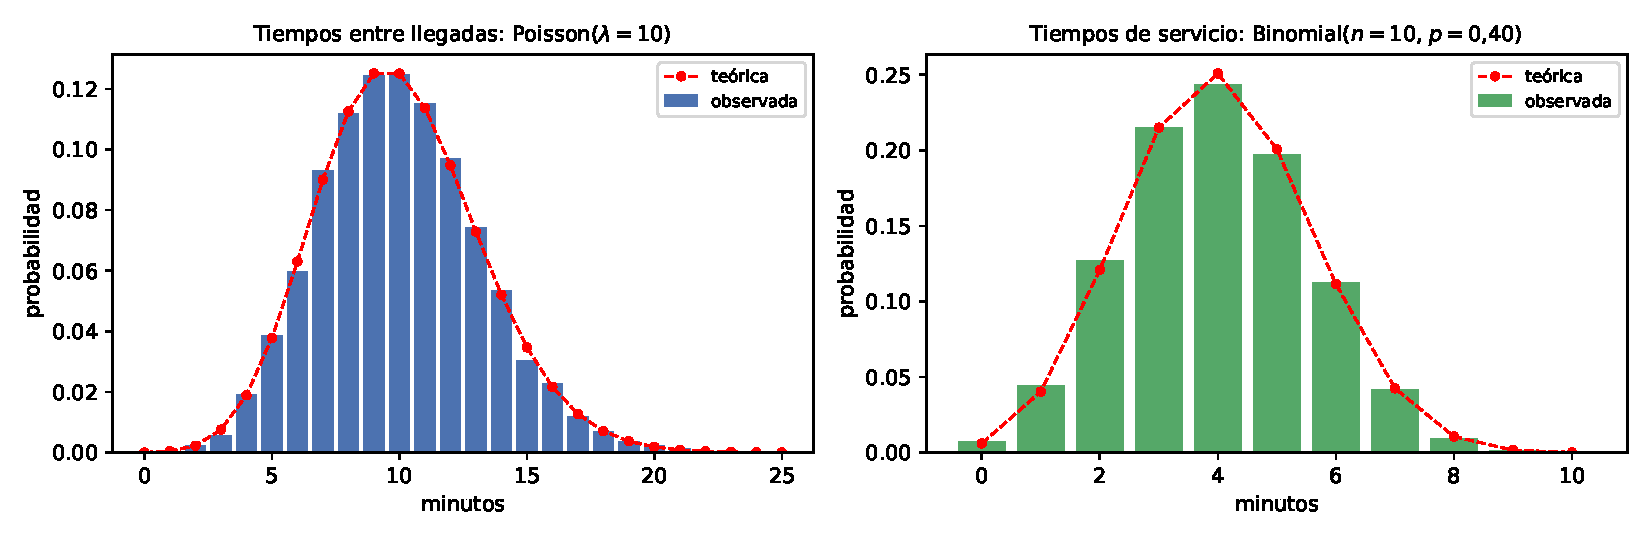
\includegraphics[width=\textwidth]{fig_pmf.pdf}
\caption{Frecuencias observadas en 10\,000 valores generados frente a las funciones de masa teóricas.}
\label{fig:pmf}
\end{figure}

\subsection{La simulación de 20 clientes}

\begin{table}[H]
\centering
\caption{Simulaci\'on \emph{ad hoc} de 20 clientes con tiempos entre llegadas Poisson($\lambda=10$) y tiempos de servicio Binomial($n=10$, $p=0{,}40$).}
\label{tab:sim20}
\small\setlength{\tabcolsep}{4pt}
\begin{tabular}{@{}rrrrrrrrr@{}}
\toprule
\makecell{(1)\\Cliente} & \makecell{(2)\\Tiempo\\entre\\llegadas} & \makecell{(3)\\Tiempo\\de\\llegada} & \makecell{(4)\\Tiempo\\de\\servicio} & \makecell{(5)\\Inicio\\del\\servicio} & \makecell{(6)\\Fin del\\servicio} & \makecell{(7)\\Tiempo en\\el sistema} & \makecell{(8)\\Tiempo\\ocioso} & \makecell{(9)\\Tiempo\\en cola} \\
\midrule
1 & --- & 0 & 4 & 0 & 4 & 4 & 0 & 0 \\
2 & 12 & 12 & 4 & 12 & 16 & 4 & 8 & 0 \\
3 & 11 & 23 & 4 & 23 & 27 & 4 & 7 & 0 \\
4 & 12 & 35 & 2 & 35 & 37 & 2 & 8 & 0 \\
5 & 12 & 47 & 3 & 47 & 50 & 3 & 10 & 0 \\
6 & 9 & 56 & 3 & 56 & 59 & 3 & 6 & 0 \\
7 & 11 & 67 & 7 & 67 & 74 & 7 & 8 & 0 \\
8 & 14 & 81 & 2 & 81 & 83 & 2 & 7 & 0 \\
9 & 9 & 90 & 1 & 90 & 91 & 1 & 7 & 0 \\
10 & 12 & 102 & 5 & 102 & 107 & 5 & 11 & 0 \\
11 & 8 & 110 & 5 & 110 & 115 & 5 & 3 & 0 \\
12 & 4 & 114 & 5 & 115 & 120 & 6 & 0 & 1 \\
13 & 12 & 126 & 3 & 126 & 129 & 3 & 6 & 0 \\
14 & 12 & 138 & 2 & 138 & 140 & 2 & 9 & 0 \\
15 & 6 & 144 & 4 & 144 & 148 & 4 & 4 & 0 \\
16 & 7 & 151 & 3 & 151 & 154 & 3 & 3 & 0 \\
17 & 7 & 158 & 3 & 158 & 161 & 3 & 4 & 0 \\
18 & 6 & 164 & 4 & 164 & 168 & 4 & 3 & 0 \\
19 & 7 & 171 & 2 & 171 & 173 & 2 & 3 & 0 \\
20 & 9 & 180 & 4 & 180 & 184 & 4 & 7 & 0 \\
\midrule
\textbf{Suma} & & & & & & \textbf{71} & \textbf{114} & \textbf{1} \\
\bottomrule
\end{tabular}
\begin{minipage}{\textwidth}\vspace{2pt}\footnotesize
Tiempo total de la simulaci\'on $T = 184$ minutos. Semillas $X_0 = 2391$ para las llegadas y $X_0 = 160005002$ para el servicio.
\end{minipage}
\end{table}

\begin{table}[H]
\centering
\caption{Medidas de desempe\~no de la corrida de 20 clientes.}
\label{tab:med20}
\small
\begin{tabular}{@{}llrl@{}}
\toprule
Medida de desempe\~no & C\'alculo & Valor & Unidad \\
\midrule
Tiempo promedio en el sistema & $\sum(7)/N = 71/20$ & 3,5500 & min \\
Porcentaje de tiempo ocioso & $\sum(8)/T = 114/184$ & 0,6196\ (61,96\%) & proporci\'on \\
Tiempo de espera promedio por cliente & $\sum(9)/N = 1/20$ & 0,0500 & min \\
Fracci\'on de clientes que esper\'o & $N_e/N = 1/20$ & 0,0500 & proporci\'on \\
Espera promedio de quienes esperaron & $\sum(9)/N_e = 1/1$ & 1,0000 & min \\
\bottomrule
\end{tabular}
\end{table}

\subsection{¿Qué puede decir de los resultados obtenidos?}

Lo primero que salta a la vista es que la cola prácticamente desapareció. De los 20 clientes solo uno
esperó, y esperó 1 minuto: el cliente 12, que llegó en el minuto 114 cuando el cajero todavía estaba
atendiendo al cliente 11 hasta el minuto 115. La columna (9) suma 1 minuto en toda la simulación. La
columna (8), en cambio, suma 114 minutos de tiempo ocioso sobre un total de 184, o sea que el cajero
estuvo desocupado el 61,96\,\% del tiempo.

Ese 61,96\,\% no es casualidad. La intensidad de tráfico del sistema es $\rho = E[S]/E[A] = 4/10 = 0{,}40$,
y la teoría dice que a largo plazo la proporción de tiempo ocioso tiende a $1 - \rho = 0{,}60$. Con
apenas 20 clientes ya se está a menos de dos puntos porcentuales de ese valor. Me parece la mejor
validación de que la simulación y los dos generadores están bien: el resultado cae donde la teoría
dice que tiene que caer, y ese número no está programado en ninguna parte, sale solo de sortear 40
valores.

Aparece además una situación que en el Laboratorio 1 no podía darse. La Binomial puede
devolver 0, y en la muestra de validación salieron 73 servicios de duración cero en 10\,000, un
0,73\,\%, que corresponde a $(1-p)^{n} = 0{,}6^{10} = 0{,}006047$ más la variabilidad del muestreo. Un
tiempo de servicio de cero minutos no tiene mucho sentido físico para un cajero de banco, y con las
uniformes discretas del Laboratorio 1 no podía pasar porque el mínimo era 1. Lo mismo aplica a la
Poisson, que en principio puede dar tiempos entre llegadas de 0, aunque con $\lambda = 10$ eso ocurre
con probabilidad $e^{-10} = 0{,}0000454$ y en 10\,000 valores no apareció ninguno.

\subsection{¿Qué similitudes o diferencias se presentan frente al Laboratorio 1?}

Para comparar en igualdad de condiciones volví a correr el modelo del Laboratorio 1, con las
uniformes discretas $U\{1,10\}$ y $U\{1,6\}$, pero alimentado por el mismo generador congruencial y
con las mismas semillas. Así lo único que cambia entre los dos modelos son las distribuciones y no la
fuente de aleatoriedad.

\begin{table}[H]
\centering
\caption{Comparaci\'on de los dos modelos sobre 10 corridas, con 20 y con 200 clientes.}
\label{tab:cmp}
\footnotesize\setlength{\tabcolsep}{4pt}
\begin{tabular}{@{}lrrrr@{\hspace{1em}}rrrrr@{}}
\toprule
& \multicolumn{4}{c}{20 clientes} & \multicolumn{5}{c}{200 clientes} \\
\cmidrule(lr){2-5}\cmidrule(lr){6-10}
Medida & \makecell{Lab 1\\media} & \makecell{Lab 1\\$S$} & \makecell{Lab 2\\media} & \makecell{Lab 2\\$S$} & \makecell{Lab 1\\media} & \makecell{Lab 1\\$S$} & \makecell{Lab 2\\media} & \makecell{Lab 2\\$S$} & Cambio \\
\midrule
Tiempo promedio en el sistema & 3,7000 & 0,5022 & 3,7300 & 0,3146 & 4,6470 & 0,5301 & 3,9980 & 0,1690 & -14,0\% \\
Porcentaje de tiempo ocioso & 0,4263 & 0,0678 & 0,6194 & 0,0302 & 0,3745 & 0,0443 & 0,6034 & 0,0191 & +61,1\% \\
Tiempo de espera promedio por cliente & 0,5300 & 0,3276 & 0,0050 & 0,0158 & 1,1890 & 0,3684 & 0,0385 & 0,0253 & -96,8\% \\
Fracci\'on de clientes que esper\'o & 0,2250 & 0,1161 & 0,0050 & 0,0158 & 0,3505 & 0,0600 & 0,0225 & 0,0106 & -93,6\% \\
Espera promedio de quienes esperaron & 2,2536 & 0,8367 & 0,1000 & 0,3162 & 3,3477 & 0,5540 & 1,5500 & 0,4529 & -53,7\% \\
\bottomrule
\end{tabular}
\begin{minipage}{\textwidth}\vspace{2pt}\footnotesize
La columna Cambio es la variaci\'on porcentual entre los dos modelos con 200 clientes. Lab 1: $U\{1,10\}$ y $U\{1,6\}$. Lab 2: Poisson($\lambda=10$) y Binomial($10$, $0{,}40$).
\end{minipage}
\end{table}

\begin{figure}[H]
\centering
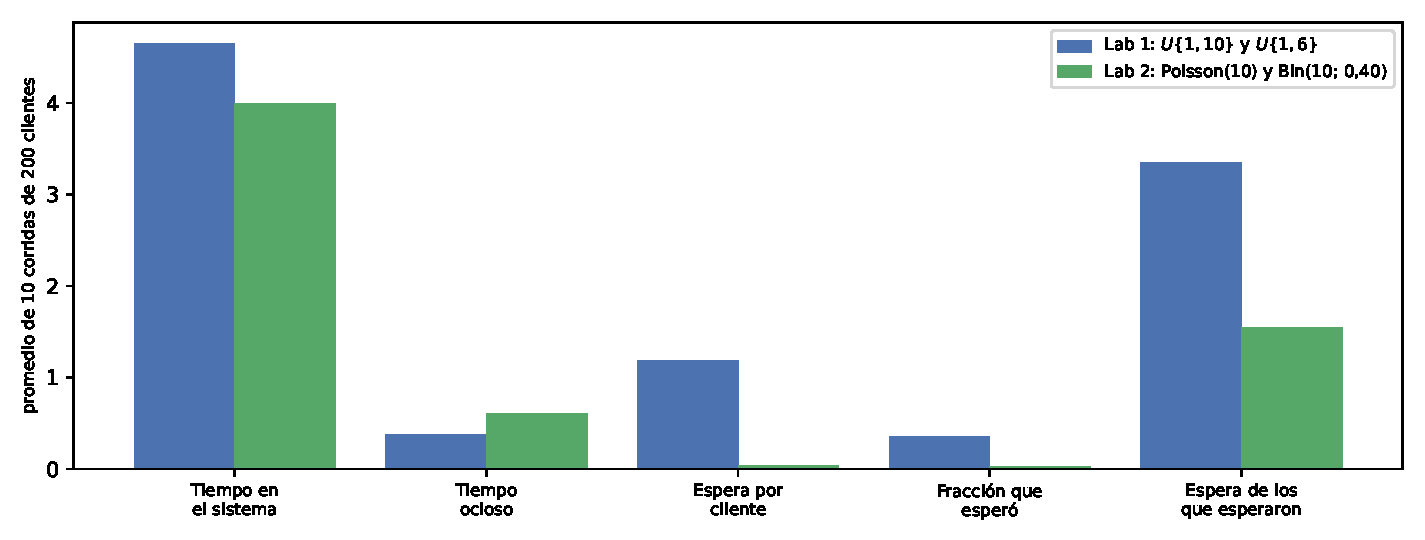
\includegraphics[width=0.92\textwidth]{fig_comparacion.pdf}
\caption{Medidas de desempeño promediadas sobre 10 corridas de 200 clientes con cada modelo.}
\label{fig:cmp}
\end{figure}

\textbf{Lo que se parece.} La estructura del modelo es la misma: un servidor, disciplina FIFO, las
mismas nueve columnas y las mismas cinco medidas. El método también, porque sigue siendo simulación
\emph{ad hoc} avanzando cliente por cliente con aritmética elemental. Lo único que se reemplazó fue de
dónde salen los dos números. De las cinco medidas, la que menos cambia es el tiempo promedio en el
sistema: 3,55 minutos aquí contra 3,45 en la corrida equivalente del Laboratorio 1, y sobre 10
corridas de 200 clientes, 4,00 contra 4,65. Tiene sentido, porque el tiempo en el sistema es servicio
más espera, y como casi nadie espera esa medida se queda pegada al tiempo de servicio promedio de 4
minutos.

\textbf{Lo que cambia.} La diferencia de fondo es la congestión. La intensidad de tráfico pasó de
$\rho = 3{,}5/5{,}5 = 0{,}636$ a $\rho = 4/10 = 0{,}400$, y eso arrastra a todas las medidas de
espera. Con 200 clientes, la espera promedio por cliente cayó 96,8\,\%, la fracción de clientes que
esperó cayó 93,6\,\% y la espera de quienes esperaron cayó 53,7\,\%. En el Laboratorio 1 esperaba uno
de cada tres clientes; acá espera uno de cada cuarenta y cinco. El tiempo ocioso medido, 0,3745 y
0,6034, reproduce casi exactamente los valores teóricos de $1-\rho$, que son 0,3636 y 0,6000.

\textbf{Un problema práctico que apareció.} Con solo 20 clientes el modelo nuevo es tan poco
congestionado que en 9 de las 10 corridas no esperó absolutamente nadie. Eso deja sin definir la
medida ``espera promedio de quienes esperaron'', porque el denominador $N_e$ vale cero. Por eso
repetí las 10 corridas con 200 clientes, y ahí sí se formó cola en las 10. Es un recordatorio de que
el tamaño de la corrida hay que elegirlo pensando en el evento que se quiere medir y no solo en el
promedio general.

\textbf{Sobre la variabilidad.} Las desviaciones estándar entre corridas también bajaron. Para el
tiempo promedio en el sistema con 200 clientes, $S$ pasó de 0,5301 a 0,1690, es decir que las
corridas del modelo nuevo se parecen mucho más entre sí. La explicación está en los coeficientes de
variación de la tabla \ref{tab:par}: los de la Poisson y la Binomial son 0,316 y 0,387, contra 0,522
y 0,488 de las uniformes discretas. Las distribuciones nuevas son relativamente menos dispersas
alrededor de su media, y en un sistema de colas la variabilidad importa tanto como el promedio para
que se formen filas.

\textbf{Una precaución sobre la comparación.} Los dos modelos no se diferencian solo en la forma de
la distribución, también en la media. Si la comparación fuera únicamente de forma habría que ajustar
las medias para dejar $\rho$ igual en los dos casos. Como la guía fija $\lambda = 10$, $n = 10$ y
$p = 0{,}40$, la diferencia de congestión viene incluida en el enunciado, y buena parte de lo que se
observa se explica por ahí y no por el cambio de familia de distribuciones.

Como comprobación adicional, el modelo del Laboratorio 1 vuelto a correr aquí con el generador
congruencial dio, sobre 200 clientes, 4,647 minutos en el sistema, 37,45\,\% de tiempo ocioso y 0,3505
de fracción que esperó. Los valores que reporté en el informe del Laboratorio 1, generados en su
momento con otra fuente de aleatoriedad, fueron 4,60, 36,07\,\% y 0,3545. Que dos fuentes distintas
den prácticamente lo mismo confirma que el motor de simulación es correcto.

% =====================================================
\section{Conclusiones}
% =====================================================

\begin{enumerate}[itemsep=4pt]

\item El tamaño de ciclo es el criterio que hay que revisar primero. Los congruenciales con $m = 128$
y $m = 48$ pasaron las tres pruebas estadísticas y aun así son inservibles, porque su periodo de 32 y
48 es menor que la muestra de 100 y el histograma les queda plano de manera trivial. Al revés, el
MINSTD con periodo de más de dos mil millones falló el Kolmogorov--Smirnov por 0,011 de diferencia. La
prueba estadística sin el periodo al lado puede llevar a la conclusión contraria.

\item Uniformidad y aleatoriedad no son lo mismo. El generador de congruencia inversa dio
$\chi^2 = 0{,}0$, es decir exactamente 10 observaciones en cada una de las 10 clases, y aun así falló
el test de rachas con $Z = 2{,}31$ por alternar valores altos y bajos. Con una sola prueba se habría
concluido que era el mejor del laboratorio.

\item En la integración Monte Carlo lo que manda es la varianza del integrando, no su complejidad. El
ejercicio 4, que tiene un integrando acotado entre 0 y 1, quedó con 1,31\,\% de error usando 100
números. El ejercicio 5, cuyo integrando va de 0,78 a 403,4, necesitó mil veces más números para
llegar a un error parecido. Y en los siete casos el error cae como $1/\sqrt{k}$, lo que obliga a
consumir muchos números y hace indispensable un generador de periodo grande.

\item El método de composición rinde cuando la función de masa se puede descomponer con una
parte uniforme. Para la distribución del literal 5.3.d bajó el costo de 6,48 comparaciones por valor
generado a 1,15, porque el 59,8\,\% de las veces resuelve el sorteo con una multiplicación y una
parte entera. El precio, consumir dos números aleatorios en vez de uno, es despreciable frente a eso.

\item Cambiar las distribuciones de entrada de la simulación cambió el sistema por completo. Pasar de
$U\{1,10\}$ y $U\{1,6\}$ a Poisson(10) y Binomial(10; 0,40) llevó la intensidad de tráfico de 0,636 a
0,400, y con eso la espera promedio por cliente cayó 96,8\,\% y la fracción de clientes que espera
pasó de uno de cada tres a uno de cada cuarenta y cinco. En los dos modelos el tiempo ocioso medido
coincidió con $1-\rho$ dentro de un punto porcentual, lo que confirma que el motor de simulación y los
generadores están bien implementados.

\item La corrida hay que dimensionarla según lo que se quiere medir. Con 20 clientes y el modelo
nuevo, 9 de 10 corridas terminaron sin un solo cliente en cola, lo que deja indefinida una de las
cinco medidas. Con 200 clientes el problema desaparece.

\end{enumerate}

% =====================================================
\section{Anexos}
% =====================================================

Se adjunta el cuaderno

\begin{center}
\texttt{Lab2\_Simulacion\_Duvan\_Baquero\_\codigoEstudiante.ipynb}
\end{center}

\noindent ejecutado de principio a fin, con el desarrollo completo de los numerales 5.1 a 5.4. Contiene las doce secuencias de números pseudoaleatorios con sus periodos y sus
tres pruebas, las siete integrales estimadas con cuatro tamaños de muestra, los 100 valores generados
en cada literal del numeral 5.3 con sus tablas de frecuencias, y la simulación \emph{ad hoc} con la
validación de los generadores de Poisson y Binomial. Todas las tablas y figuras de este informe salen
de ese cuaderno.

% =====================================================
\begin{thebibliography}{9}

\bibitem{ross99}
Ross, S. \emph{Simulación}, 2.\textsuperscript{a} edición. Pearson Press, 1999. Capítulos 3 y 4.

\bibitem{banks1998}
Banks, J. \emph{Handbook of Simulation: Principles, Methodology, Advances, Applications, and
Practice}. John Wiley \& Sons, Inc., 1998. Capítulo 1.

\bibitem{mancilla2000}
Mancilla Herrera, A. M. \emph{Números aleatorios. Historia, teoría y aplicaciones}. Ingeniería y
Desarrollo, núm. 8, diciembre de 2000, pp. 49--69. Universidad del Norte, Barranquilla, Colombia.

\end{thebibliography}

\end{document}
